\section{Motion Control}
\index{control}
We human can carefully plan our motion, coordinately and purposeful exercise our muscles to achieve a wide variety of high-level tasks, ranging from simple locomotion, dexterous hand manipulation, to highly skillful stunts. To model them in animation, simulating the passive dynamics is not enough. The key challenge that motion control tackles is to find controllers that can achieve high-level motion tasks (e.g. walk at 1 m/s, grasp a bottle and open the cap, etc.). In character animation, a controller is the character's ``algorithmic brain'' that decides how much torque ($\boldsymbol{\tau}^a$ in eq. \ref{eq:dynamics} and \ref{eq:generalized}) are needed at each joint to successfully fulfill the task in a way that mimics human behavior. Optimization-based motion control is the most extensively researched topic in physically-based character animation. The optimization searches for a controller that minimizes a task-related cost function, subject to dynamical constraints.

\begin{figure}[h]
  \centering
  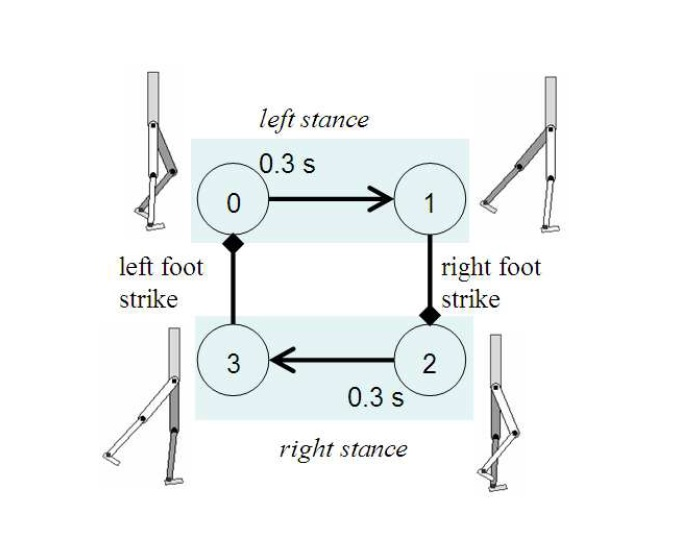
\includegraphics[width=0.55\textwidth]{figures/stateMachine.jpg}
  \caption{Different stages of walking in SIMBICON. Image courtesy of \cite{Yin:2007}.}
  \label{fig:stateMachine}
\end{figure}

One common misunderstanding is that one can formulate a large optimization for arbitrary tasks. Due to complexity of human motions and nonlinearity of the dynamics, a large optimization may have competing objectives and many local minima. Up till today, there is no efficient optimization algorithms that can reliably find meaningful controllers in such cases. For this reason, a common practice in this field is to decompose a high-level task into multiple lower-level subtasks and formulate smaller optimization for each of the simpler subtask. For examples, In SIMBICON \cite{Yin:2007}, a walking cycle is decomposed into multiple stages (Figure \ref{fig:stateMachine}). Within each stage, separate optimizations can be used for controlling the two legs, the upper body, the balance and the style. After solving all the optimizations, these low-level controllers can be combined so that the character can walk naturally and robustly. Controller decomposition depends on the task and requires domain knowledge. We refer the readers to the research literature to learn controller decomposition on a case-by-case basis. In this section, we will discuss two generic optimization-based methods of motion control: trajectory optimization and reinforcement learning. 



\subsection{Trajectory Optimization}
\index{trajectory optimization}
Starting from the classical paper ``Spacetime Constraints''\index{spacetime constraints} \cite{Witkin:1988}, trajectory optimization has become a mainstream technique in physically-based character animation. It searches for a controller that minimizes a cost function subject to physical constraints. The general form of the optimization is:
\begin{equation}
  \begin{array}{cl}
    \min_{\vc{x},\vc{u}}&\sum_{t=0}^{N}g(\vc{x}_t,\vc{u}_t)\\
    \textrm{subject to}&\\
    &\vc{x}_{t+1}=\vc{h}(\vc{x}_t)+\vc{B}_t\vc{u}_t
  \end{array}
  \label{eq:trajectoryOptimization}
\end{equation}
where $\vc{x}$ is the physical states and $\vc{u}$ is the control. In character animation, the states are usually defined as $\vc{x}:=\vc{[q, \dot{q}]}^T$ and the control $\vc{u}:=\boldsymbol{\tau}^a$. $g$ is the cost function, which is hand-crafted to reflect the high-level task. For example, if the task is to walk at 1 m/s, one term in the cost function could be the distance between the current COM of the character and a desired COM position that moves at 1 m/s. The constraint usually consists of the dynamics equations $\vc{h}$. Note that in most applications of character animation, the dynamics are nonlinear to the state $\vc{x}$ but linear to the control $\vc{u}$ (see eq. \ref{eq:dynamics} and \ref{eq:generalized}). In addition, the constraints can also include joint limits, torque limits, and other task-related requirements.

To make it more concrete, we will revisit the simple example in the original ``Spacetime Constraints''\index{spacetime constraints} paper: controlling a single particle. The task of this particle is to fly from point $\vc{a}$ to point $\vc{b}$ in $T$ seconds using a time-varying jet force $\vc{f}(t)$. The dynamics of the particle is $m\vc{\ddot{x}}-\vc{f}-m\vc{g}=0$, where $\vc{x}$ is its position, $m$ is its mass and $\vc{g}$ is gravity. The goal of this flight is to minimize the total fuel consumption $\int_0^T|\vc{f}|^2dt$. After discretization along time, the optimization has the following form:
\begin{displaymath}
  \begin{array}{cl}
    \min_{\vc{x},\vc{f}}&\sum_{t=0}^{N}|\vc{f}_t|^2\\
    \textrm{subject to}&\\
    &\vc{x}_{t+1}= 2\vc{x}_{t} -\vc{x}_{t-1}+\frac{\Delta t^2}{m}\vc{f}_t+\Delta t^2\vc{g}\\
    &\vc{x}_0=\vc{a}\\
    &\vc{x}_N=\vc{b}
  \end{array}
  \end{displaymath}

It is not too difficult to extend the above derivations to control a human character. We will need to change the control force $\vc{f}(t)$ to joint torques $\boldsymbol{\tau}^a(t)$, the physical constraint to the dynamics equation of articulated rigid bodies (eq. \ref{eq:dynamics} or \ref{eq:generalized}), and the cost function to a relevant function specific to the task.

There are different options to solve the optimization according to the structure of the problem. Assuming the cost function and the dynamics equations are smooth, \citet{Witkin:1988} applied a generic nonlinear optimizer, Sequential Quadratic Program (SQP)\index{SQP}, to solve the problem. It is an iterative optimization technique that solves a sequence of quadratic programs that approximate the original problem. The solution of SQP is an optimal trajectory of state $\vc{x}^*(t)$ and control $\vc{u}^*(t)$. Note that this method produces a \emph{feedforward}\index{feedforward} (open-loop) controller: a trajectory over time. It cannot be generalized to the neighboring regions of the state space. As a result, the controller will fail the task even with a slight disturbance to the motion.

When the cost function is quadratic and the dynamics equation is linear,
\begin{equation}
  \begin{array}{cl}
    \min_{\vc{x},\vc{u}}&\sum_{t=0}^{N}\vc{x}_t^T\vc{Q}_t\vc{x}_t+\vc{u}_t^T\vc{R}_t\vc{u}_t\\
    \textrm{subject to}&\\
    &\vc{x}_{t+1}=\vc{A}_t\vc{x}_t+\vc{B}_t\vc{u}_t
  \end{array}
  \label{eq:LQR}
\end{equation}
the trajectory optimization is called an LQ problem. This problem can be solved very efficiently by linear-quadratic regulator (LQR)\index{LQR}. The derivation of LQR can be found in most of optimal control textbooks \cite{todorov2006optimal}. Thus we will not repeat it here. The solution is a \emph{feedback}\index{feedback} (close-loop) controller $\vc{u}_t=\vc{K}_t\vc{x}_t$. Although the requirement of linear dynamics seems restrictive, LQR still plays an important role in physically-based character animation. One important application is to design a physically-based controller to track motion captured data, which is an effective way to increase the realism of the synthesized motions. Given a motion capture\index{motion capture} sequence $\vc{\bar{x}}$, we can linearize the dynamics equation at its vicinity:
\begin{displaymath}
  \Delta \vc{x}_{t+1}=\frac{\partial \vc{h}}{\partial \vc{x}}\Delta \vc{x}_{t}+\vc{B}_t\vc{u}_t+\vc{h}(\vc{\bar{x}}_t)-\vc{\bar{x}}_{t+1}
  \end{displaymath}
where $\Delta \vc{x}=\vc{x}-\vc{\bar{x}}$. This gives an LQ problem that seeks a feedback\index{feedback} controller $\vc{u}_t=\vc{K}_t\Delta \vc{x}_t$ that minimizes the difference between the actual and the reference motion over the entire trajectory.

More importantly, LQR is a building block to solve the more general trajectory optimization problem (eq. \ref{eq:trajectoryOptimization}). Given an initial trajectory $\vc{x}_0, \vc{u}_0, \vc{x}_1, \vc{u}_1, ... , \vc{u}_N, \vc{x}_N$, we can perform the following steps iteratively:
\begin{enumerate}
\item{Compute the LQ approximation of the original problem (\ref{eq:trajectoryOptimization}) around the current trajectory by computing a first-order Taylor expansion of the dynamics, and a second-order expansion of the cost function.}
\item{Use LQR to solve the LQ approximation to get an optimal controller.}
\item{Apply the current optimal controller to generate a new trajectory.}
  \item{Go to Step 1 until convergence.}
\end{enumerate}
This iterative-LQR process\index{iterative-LQR} is similar to the core idea behind differential dynamic programming (DDP)\index{DDP}. We refer the interested reader to \citet{todorov2006optimal} for a more thorough discussion about LQR and DDP. The key advantage of DDP is that it not only provides a feedforward trajectory, but also an optimal feedback controller near that trajectory.

To sum up, trajectory optimization is an effective way to synthesize character animation. The synthesized motion is not only physically correct, but more importantly, demonstrates an important animation principle, anticipation. This is because the objective of trajectory optimization is to minimize a long-term cost. Thus, the character can move intelligently that gives up short-term gains to minimize the long-term cost. For example, for a jump-up task, the trajectory optimization could produce a controller that sacrifices the height of the character's COM first for a much higher jump later. However, there are a few shortcomings of trajectory optimization. First, it often leads to a high dimensional optimization that is expensive to solve. Another problem of high dimensional nonlinear optimization is that the solver is more likely to get stuck at bad local minima. Thus, a good initialization is extremely important. Last but not least, trajectory optimization exploits the mathematical form of dynamic equations to design the optimal controller. If the dynamics is not smooth, too complicated or unknown, it is not clear how to apply trajectory optimization methods.


\subsection{Reinforcement Learning}
\index{reinforcement learning}
Reinforcement learning is motivated by the learning process of humans. It optimizes a controller by interacting with the physical environment with numerous trials. Initially, the controller tries out random moves. If a desired behavior is observed, a reward is provided as the positive reinforcement. This reward system will gradually shape the controller until eventually it successfully fulfills the high-level task. Reinforcement learning is an active research area, with a large number of algorithms proposed every year. We refer readers to \cite{Kaelbling1996,Bagnell:2013} for a thorough review. We will focus on policy search\index{policy search} in the remaining of this section. Policy search is a popular reinforcement learning algorithm in physically-based character animation. It performs extremely well in this field because it can solve control problems with high-dimensional continuous state and action spaces, which is essential to control a human character. 

Mathematically, reinforcement learning solves a Markov Decision Process (MDP)\index{MDP}. An MDP is a tuple $(S, A, R, D, \gamma, P_{sas'})$, where $S$ is the \emph{state}\index{state} space; $A$ is the \emph{action}\index{action} space. The states reflect what the current situation is and the actions are what a character can perform to achieve the specified task. $R$ is the \emph{reward function}\index{reward function}. A reward function is a mapping from the state-action space to a real number: $R: S\times A\mapsto \mathbb{R}$, which evaluates how good the current state and action are. $D$ is the distribution of the initial state $s_0 \in D$ and $\gamma \in [0, 1]$ is the discount factor of the reward over time. $P_{sas'}$ is the \emph{transition probability}\index{transition probability}. It outputs the probability that the next state is $s'$ if an action $a$ is taken at the current state $s$. In physically-based character animation, the transition probability is computed by physical simulation. Although most of the physical simulations are deterministic, random noise can be added in simulation to increase the robustness of the learned controller \cite{Wang:2010}.

The solution of an MDP is a control \emph{policy}\index{policy} $\pi$ that maps the state space to the action space $\pi: S\mapsto A$. It decides what actions to take at different situations. The \emph{return} of a policy is the accumulated rewards along the state trajectory starting at $s_0$ by following the policy $\pi$ for $N$ steps.
\begin{displaymath}
V^\pi(s_0)=\sum_{i=0}^N{\gamma^{N-i}R(s_i, \pi(s_i))}
\end{displaymath}
The reward at earlier states can be exponentially discounted over time. The \emph{value} of a policy is the expected return with respect to the random initial state $s_0$ drawn from D.
\begin{equation}
V(\pi)=E_{s_0\sim D}[V^\pi(s_0)]
\label{eq:policyValue}
\end{equation}
Note that the goal of MDP is not to maximize the short-term reward $R$ at the next state, but a long term value function $V$. Using $V$ instead of $R$ as the optimization target prevents the controller from applying short-sighted greedy strategies. This agrees with our ability of long-term planning when we are executing our motions.

To formulate an MDP, we need to design the state space $S$, the action space $A$, the reward function $R$ for a given task. Ideally, the state space should contain all the possible states of the articulated rigid body system, including the joint angles $\vc{q}$, joint velocities $\dot{\vc{q}}$ and time $t$, and the actions should include all the joint torques $\vc{\tau}^a$. However, this means that the state and the action space can have hundreds of dimensions. Due to the \emph{curse of dimensionality}, solving an MDP in such a high dimensional continuous space is computational infeasible. In practice, researchers often carefully select states and actions specifically for the tasks in question to make the computation tractable. For example, if the task is to keep balance while standing. The state space only needs to include important features for balance, such as the character's COM and the center of the ground contact polygon. Similarly, given the well-known balance strategies, such as ankle strategy and hip strategy, the action space can be as simple as a few torques at lower body joints. Using prior knowledge\index{prior knowledge} of the task can greatly simplify the problem, which is a common practice in physically-based character animation. 

A reward function for character animation usually consists of two parts, a task-related component that measures how far the current state is from the goal state and a component that evaluates the naturalness of the motions. Designing a good reward function is essential to the success of the entire learning algorithm. A good design of the reward should be a smooth function that gives continuous positive reinforce whenever progress is made. Mathematically, this design will present gradient information that can guide optimization solvers. In contrast, a common mistake is to give reward only when the task is achieved, which makes the reward function a narrow spike and flat zero elsewhere. This should be avoided because nearly all the optimization algorithms would have trouble finding such a spike.

To apply policy search to solve the MDP, we need to parameterize the policy\index{policy parameterization}. A policy can be any arbitrary function. A practical way to optimize it is to parameterize it and then search for the optimal policy parameters. Commonly-used parameterizations include look-up tables, linear functions, splines and neural networks. Parameterization determines the potential quality of the final policy. However, there is no consensus what the best way is to parameterize a policy. It is decided on a case-by-case basis. Once the policy parameterization is decided, an initial policy is iteratively evaluated and improved until the optimization converges or a user-specified maximum number of iterations is reached.

To evaluate a policy\index{policy evaluation}, we can execute the policy in the simulation for N time steps with different initial states $s_0\in D$, accumulate the rewards and average the returns to compute the value of the policy. Policy improvement adjusts the policy parameters to increase its value. A straightforward way is to follow the policy gradient \cite{Ng:2000:PPS}. However, in many character animation tasks, such as locomotion and hand manipulation, contact events happen frequently, which introduces unsmooth contact forces that invalidate policy gradient. For this reason, sample-based stochastic optimization techniques are particularly suited for physically-based character animation. Covariance Matrix Adaptation Evolution Strategy (CMA-ES)\index{CMA-ES} \cite{hansen2006cma} is the most frequent applied optimization methods for motion control. CMA can work as long as we can evaluate the value of the policy. It does not need to compute gradient and does not rely on good initializations. More importantly, CMA is a ``global'' search algorithm that explores multiple local optima. Although there is no guarantee that CMA will converge at the global optimum, in practice, it often finds good local optima in moderately high dimensional control spaces (\eg 20-30 dimensions). For the completeness of the chapter, we will briefly describe the CMA algorithm. Readers can refer to the original paper \cite{hansen2006cma} for additional details.

CMA starts with an initial underlying Gaussian distribution in the policy parameter space with a large covariance matrix. A population of samples is drawn from this distribution. The first generation of samples are not biased in the parameter space due to the large covariance matrix. Each CMA sample represents a control policy. The policies are evaluated through simulation. They are sorted according to their values and a certain percentage of the inferior samples are discarded. The underlying Gaussian distribution is updated according to the remaining good samples and is used to generate the next generation of the samples. This process is performed iteratively. Over iterations, the underlying distribution is shifted and narrowed. Eventually, the distribution converges to a good region of the policy space. The best CMA sample throughout all the iterations is selected as the optimal control policy.

In summary, reinforcement learning is a generic method for motion control. It can automatically learn a wide range of behaviors through simulation trials. Reinforcement learning, more specifically, policy search\index{policy search}, is becoming one of the most popular approaches in character animation synthesis. Reinforcement learning does not assume any mathematical forms of the dynamics equation. It treats the physical simulation as a black box, as long as it can output the next state given the current state and action. Thus, it is not bounded to a particular dynamics model. The same learning algorithm can still work even if the simulation software is upgraded. The main challenge of reinforcement learning is to design the states, the actions, the reward and the policy parameterization. We need to inject enough prior knowledge\index{prior knowledge} into the design so that the search space is small enough to be computationally feasible, but not too small to contain effective policies. This requires a lot of experience and manual tweaking, especially for challenging motion tasks. 
